\subsection{Cosmic Radiation Methods}
\label{sec:Cosmic-Radiation-Methods}

The Timepix sensors output data in a human-readable, array-like format that directly corresponds to the pixel array of the sensor.
The sensor collects data in a manner similar to that of an optical camera.
A shutter time is a parameter defined by the user, and the sensor will collect data for the entire duration of the shutter time.
Once the time has lapsed, the sensor packages the data into a data frame and is sent to the storage of the computer.
The length of the shutter time must be carefully chosen.
Too short of a length will result in many empty data frames that waste storage space, but too long of a length will result in data frames which are unreadable since the particle tracks in the frame will be indistinguishable from one another.
Each pixel in the 256 by 256 sensor array has one corresponding energy value per frame, so this array can be used to reconstruct the data frame.
The energy threshold is another user-defined parameter that determines the minimum energy which can be detected by the sensor.
The primary purpose of the energy threshold is to filter out extraneous whitenoise from the environment.
<< FINISH THIS: Add the energy threshold and the shutter time used for the devices in the mission >>
An example of a data frame can be seen in Figure \ref{fig:minipix-example-frame}
A separate file contains the metadata for each data frame, and contained within the metadata is information such as the energy threshold and the timestamp.

\begin{figure}[h!]
	\begin{center}
		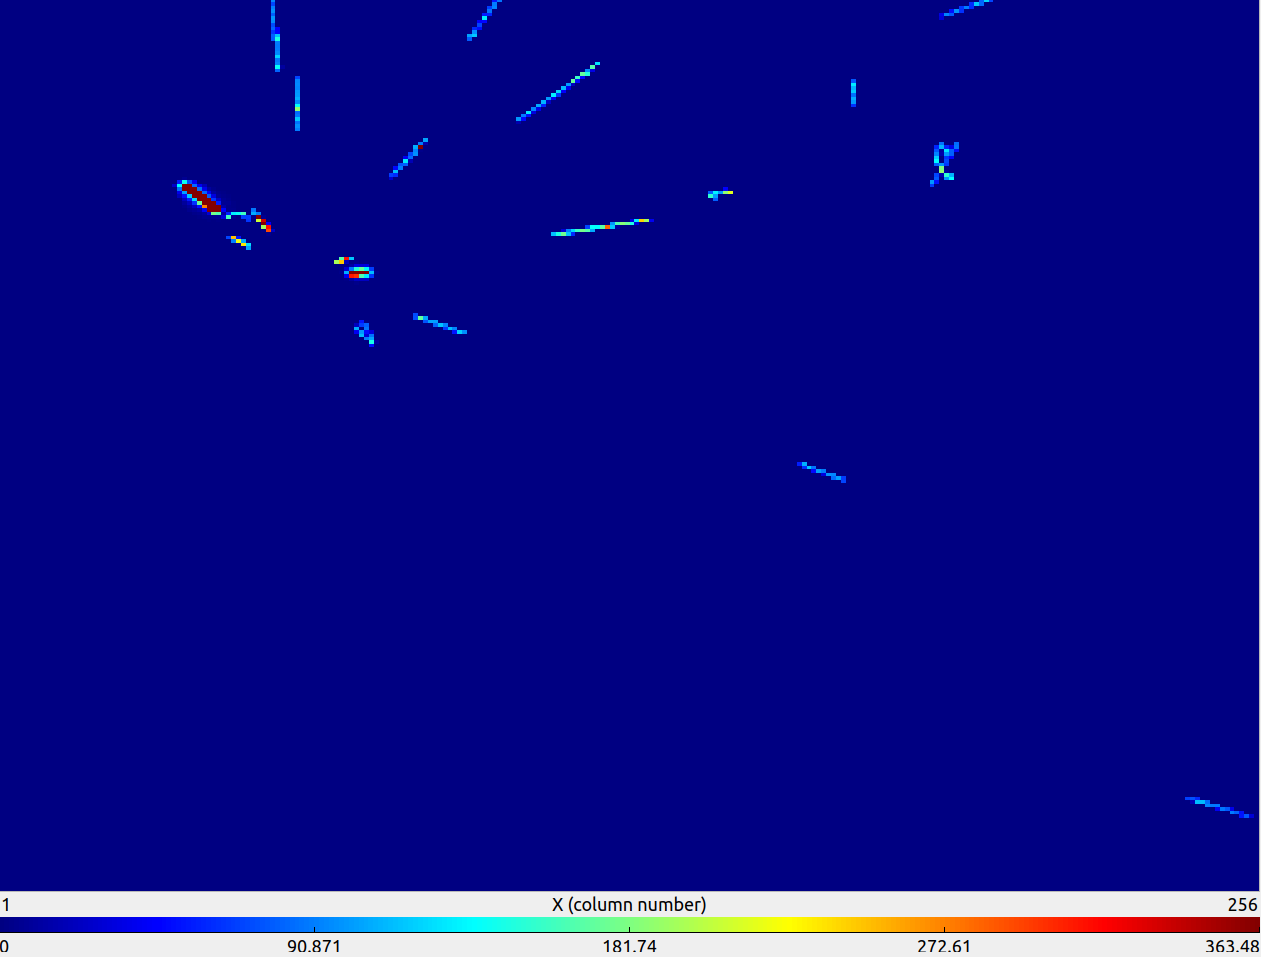
\includegraphics[width=\textwidth]{figures/interesting-frame-3447.png}
		\caption{Example of a Timepix data frame. This is one of the MiniPIX data frames from the 2019 mission.}
		\label{fig:minipix-example-frame}
	\end{center}
\end{figure}

% Detail the analysis techniques used to determine the morphology and the dose (see 2018 report)

%To analyze the Timepix output, a couple of parameters regarding the sensor itself are required.
Using the techniques detailed by Jakubek et. al. \cite{Jakubek-Analysis}, the radiation dose deposited in the sensor by a particle can be calculated using the following equation
\begin{equation*}
  D_{Si} = \dfrac{E}{M_d},
\end{equation*}
where $E$ is the total energy that a particle deposited into the sensor and $M_d$ is the mass of the sensor.
It is important to note that this dose value is not the same as dose deposited in human flesh, which is referred to as dose equivalent.
Conventional calculations for dose equivalent in tissue requires use of Monte Carlo simulations to calculate a conversion factor \cite{Stuart-Thesis} and is outside the SORA missions' scope of study.
%This computation prevents the real-time calculation of dose that was performed in the SORA missions. 
Calculating the total energy of a particle requires the use of a clustering algorithm.
The clustering algorithm analyzes the raw matrix output from the Timepix sensor and groups the pixels with non-zero energy into clusters, or tracks.
The total energy of the cluster, $E$, is the sum of all pixel energies in the cluster.

%This analysis method is relatively simple to understand, but the techniques required to compute the clusters is rather complex.
Another property of interest from the Timepix data is the linear energy transfer (LET), which provides a standard with which all particle clusters can be examined independent of the particle's incident angle.
%This is particularly important with Timepix sensors since the particle's zenith angle cannot accurately be determined. 
To calculate the LET in the silicon sensor, the following relation is used
\begin{equation*}
  LET_{Si} = \dfrac{E}{L},
\end{equation*}
where $E$ is the same energy value used in the $D_{Si}$ calculation, and $L$ is the length of the track in the detector in three dimensions.
The clustering algorithm uses a typical flood-fill technique to group touching pixels with non-zero energy.
A minimum-area bounding box is then constructed around the cluster with a linear least square fit line which intersects the bounding box, and the projected track length $L_p$ is taken to be the length of the linear least square fit line.
A visual example of the bounding box and the linear least square fit line can be seen seen in Figure \ref{fig:stuart-track-example}.
\begin{figure}[h!]
	\begin{center}
		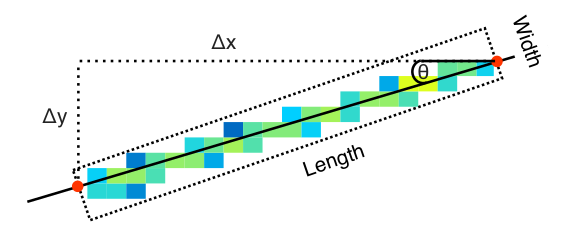
\includegraphics[width=0.75\textwidth]{figures/stuart-track-example.png}
		\caption{A visual from Ref. \cite{Stuart-Thesis} which shows the minimum-area bounding box (the dotted black box surrounding the particle track) and the linear least square fit line (the solid black line running along the particle track).}
		\label{fig:stuart-track-example}
	\end{center}
\end{figure}
$L$ can now be calculated using $L_p$ and $T$, the thickness of the sensor with
\begin{equation*}
  L = \sqrt{L_p^2 + T^2}.
\end{equation*}
Since $T$ is a known property of the sensor, the LET value can then be calculated on a per particle basis.
While out of the scope of the SORA 3 studies, the LET is a value used in calculating the dose equivalent in human flesh.

The primary method of categorizing the particle incident on the detector is by the morphology of the resulting cluster.
The track seen in the detector data will change its shape depending on the energy and the type of the particle.
The actual identity of the incident particle cannot be directly measured by the sensor, but an inference can be made by using the energy and shape of the cluster. Ref. \cite{Stuart-Thesis} gives some examples, stating that heavy tracks often correspond to high energy protons and alpha particles, medium blobs can correspond to very slow charged particles, straight tracks can be caused by light minimum ionizing particles (e.g. muon, pion). and light tracks can be caused by electrons and positrons.     
Figure \ref{fig:stuart-track-types} shows the classifications used in the SORA experiments.
\begin{figure}[h!]
	\begin{center}
		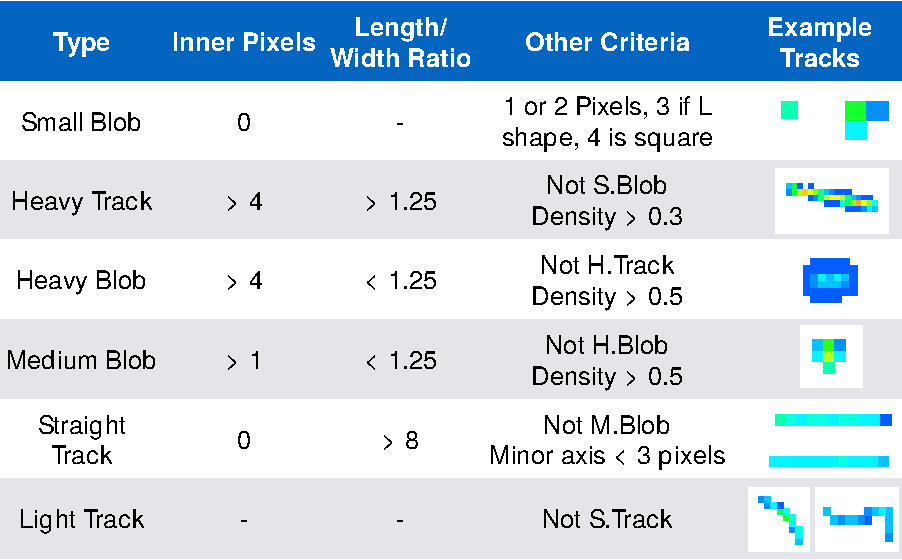
\includegraphics[width=\textwidth]{figures/stuart-track-types.pdf}
		\caption{A visual from Ref. \cite{Stuart-Thesis} showing the categories of tracks. This classification system is the same that is used in the SORA experiments.}
		\label{fig:stuart-track-types}
	\end{center}
\end{figure}

\subsection{Organic Solar Cell Methods}
\label{sec:Solar-Cell-Methods}

In order to emulate lab results of solar cell characterization as best as possible in a near space environment a current-to-voltage converter was constructed [reference figure]. A digital potentiometer, MPC4131, was used to apply a bias voltage across a solar cell which would produce a current in the micro-Amp range. A combination of two LM2904 operational amplifiers were required to capture both positive and negative current readings which were read as analogue values by the Arduino MEGA. The circuit diagram can be seen in Figure \ref{fig:solar-cell-circuit}

\begin{figure}[h!]
	\begin{center}
		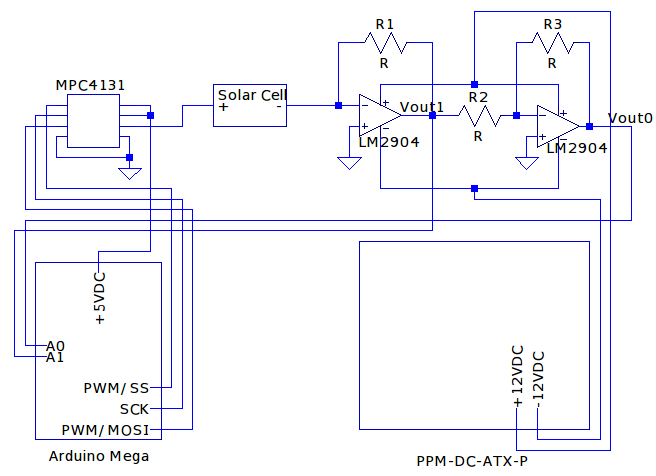
\includegraphics[width=0.75\textwidth]{figures/solar-cell-circuit-diagram.png}
		\caption{Circuit diagram of the current-reading circuit constructed for the solar cells.}
		\label{fig:solar-cell-circuit}
	\end{center}
\end{figure}
